\chapter{Introduction}
\label{chapter:introduction}

Program synthesis is the problem of automatically generating program
\textit{implementations} from high-level \textit{specifications}.
Amir Pnuelli, former computer scientist and Turing Award, described it as ``one
of the most central problems in the theory of
programming''~\cite{Pnueli:1989:ARM}, and it has been portrayed as one of the
holy grails of computer science~\cite{Solar-Lezama:2008,Gulwani2017}.
It is easy to understand why: if only we could tell the computer \textit{what to
do} and let it figure out \textit{how to do} it, the task of programming would
be so much easier!
However, Program synthesis is a very hard problem.
Programming is a task that is hard for humans and, given its generality,
there is no reason to believe it should be any easier for computers.
Computers lack algorithmic insight and domain expertise.
Moreover, the challenge is actually twofold: we need to find out both how to
tackle the intractability of the program space, and how to accurately capture
user intent~\cite{Gulwani2017}.

It is important to have in mind that program synthesis is not a panacea for
solving problems in computer programming.
For example, we might be interested in other properties besides functional
correctness, such as efficiency or succinctness of the generated program.
Also, in the general case, it is impossible for program synthesis to eliminate
all sources of bugs.
Particularly, it cannot solve problems originating from bad specifications
that come from a poor understanding of the problem domain.

Writing specifications is, indeed, a delicate process.
This might be better understood with a simple, yet non-trivial, example.

\section{Example: Sorting}
\label{sec:sorting-example}

In order to exemplify how the interaction between the user and the computer
(from now on referred to as the ``synthesizer'') might occur, let us suppose we
are interested in developing a sorting procedure, \lstinline{sort}, for lists of
integers:

\begin{lstlisting}[xleftmargin=.2\textwidth]
  sort: (xs: List Int) -> (xs': List Int)
  sort([])    = []
  sort(x::xs) = insert(x, sort(xs))

  insert: (x: Int, xs: List Int) -> (xs': List Int)
  insert(x, [])    = [x]
  insert(x, y::ys) = if x <= y then (x::y::ys)
                               else y::insert(x, ys)
\end{lstlisting}

\noindent
The function \lstinline{sort} would take a list of integers as input and return
it sorted in ascending order. One approach to implement \lstinline{sort} is to
resort to an auxiliary function, \lstinline{insert}, taking an element
\lstinline{x} and a list \lstinline{xs} as inputs, and returning a new list
\lstinline{xs'}. Assuming that \lstinline{xs} is sorted, \lstinline{insert}
guarantees that \lstinline{xs'} is also sorted by placing \lstinline{x} in the
``right place''. It is easy to see, by induction, that \lstinline{sort} is
correctly defined.

Nevertheless, it would be nicer if we could just give the synthesizer a
specification of what it means for a list to be sorted and let it figure out the
implementation. For example, the synthesizer could support using type signatures
and predicates as specifications. We could also hint the structure of the
implementation to the synthesizer by giving a specification for another
function, \lstinline{insert}, which we could believe to be useful to implement
\lstinline{sort}:

\begin{lstlisting}[xleftmargin=.2\textwidth]
  isSorted: List Int -> Bool
  isSorted([])       = True
  isSorted([x])      = True
  isSorted(x::y::ys) = x <= y and isSorted(y::ys)

  sort: (xs: List Int) -> (xs': List Int)
  sortSpec: isSorted(xs')

  insert: (x: Int, xs: List Int) -> (xs': List Int)
  insertSpec: isSorted(xs) ==> isSorted(xs')
\end{lstlisting}

\noindent
There is a problem with our specification, however, as there are many unwanted
programs that satisfy it.
The program that ignores its input and simply outputs the empty list is one such
example.
The problem is that the specification does not model our intent precisely.
It should be clear that the output \lstinline{xs'} should be in some way related
to the input \lstinline{xs}, but the current specification does not capture that
relation.
We must require that \lstinline{xs'} has exactly the same contents as those of
\lstinline{xs}, meaning that every element of \lstinline{xs} should appear in
\lstinline{xs'} in the same amount.
We could express that requirement as a binary predicate \lstinline{sameContents}
over lists (whose implementation is omitted) and add it to specification:

\begin{lstlisting}
  sort: (xs: List Int) -> (xs': List Int)
  sortSpec: isSorted(xs') and sameContents(xs, xs')

  insert: (x: Int, xs: List Int) -> (xs': List Int)
  insertSpec: isSorted(xs) ==>
    isSorted(xs') and sameContents(xs', x::xs)
\end{lstlisting}

It should be clear by now why writing specifications can be tricky, even in
simple cases.
What might be less clear is that the specification as it is might still not be
fully specified.
There are countless other properties that we might want our sorting procedure to
satisfy, such as, for example, stability, complexity, or adaptability.

\section{OutSystems and \Glsfmtfull{pbe}}
\label{sec:outsystems-pbe}

This work was done during an internship at
OutSystems.~\footnote{\url{https://www.outsystems.com}} 
OutSystems is also the name of a low-code platform that features visual
application development, easy integration with existing systems, and the
possibility to add own code when needed.

\begin{figure}
  \centering
  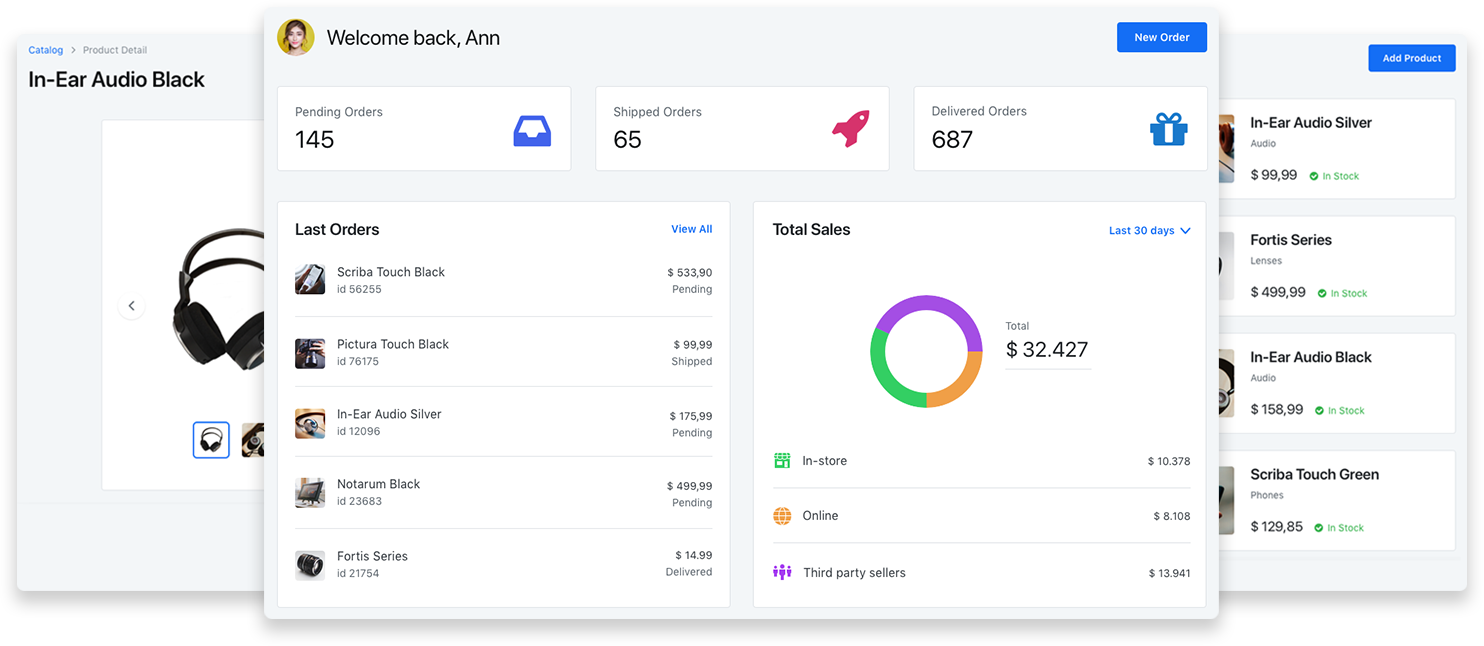
\includegraphics[width=1.0\textwidth]{assets/outsystems-app.png}
  \caption{An application developed with the OutSystems platform.}
\end{figure}

\begin{figure}
  \centering
  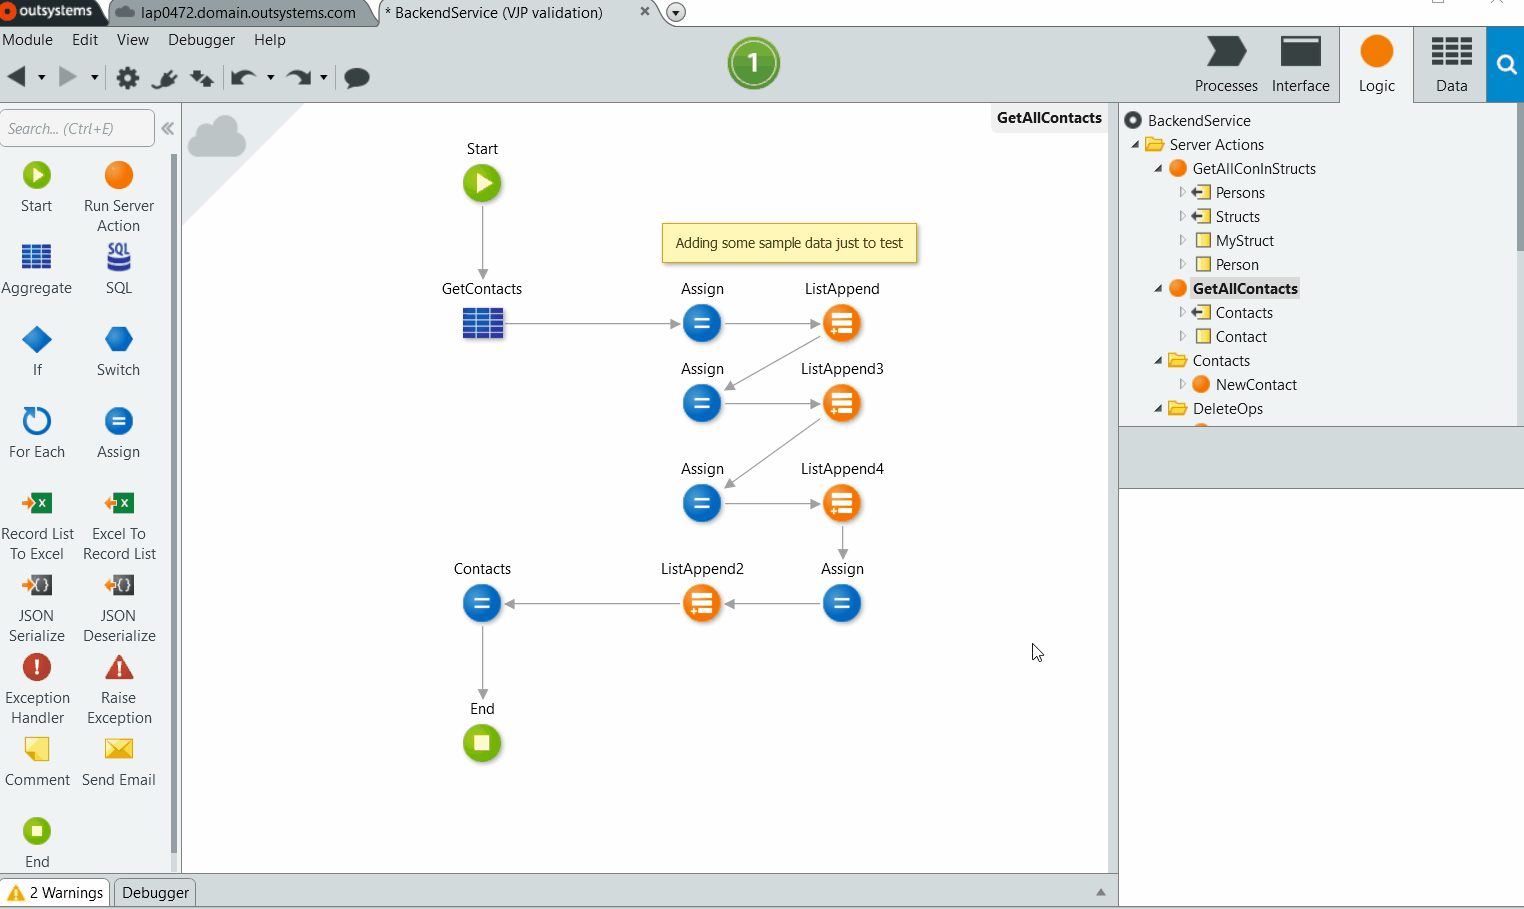
\includegraphics[width=1.0\textwidth]{assets/outsystems-studio.png}
  \caption{A screenshot of the OutSystems Service Studio integrated development
    environment. Service Studio is part of the OutSystems platform.}
\end{figure}

\noindent
With OutSystems one should be able to build enterprise-grade applications
swiftly and with a great degree of
\textbf{automation}.~\footnote{\url{https://www.outsystems.com/platform/}}
To that effect, the kind of programs we are interested in are expressions in the
OutSystems language
\footnote{\url{https://success.outsystems.com/Documentation/11/Reference/OutSystems_Language/Logic/Expressions}}.

\begin{example}\label{ex:intro:first-name}
  Suppose that, given a text representing a person's name, we are interested in
extracting the first name and prepend it with a prefix. For example, given the
text ``John Michael Doe'' and the prefix ``Dr. '' we would like to obtain
``Dr. John''. The following expression satisfies the specification.
 
\begin{lstlisting}
  prog(name, prefix) = Concat(prefix,
                              Substr(name, 0,
                                     Index(name, " ", 0)))
\end{lstlisting}
\end{example}

Thus, we were interested in building a synthesizer for OutSystems expressions
that would be \textit{performant} and \textit{easy to use}.
This would imply that the synthesis process should finish in a matter of seconds
(instead of hours or days), and the synthesizer should have a
``push-button''-style interface that does not force the user to acquire new
skills.
The paradigm in program synthesis that best fits this scenario is called
\glsfmtfull{pbe}.
In \gls{pbe}, the synthesizer should be able to synthesize ``correct'' programs
merely from a small set of input-output examples.
For instance, one possible input-output example for the program from
example~\ref{ex:intro:first-name} is, for example, (<``John Michael Doe'', ``Dr.
''>, ``Dr. John'').
By correct we mean that the program matches what the user had in mind.

The most notable success in the area of program synthesis is incorporated in a
tool called FlashFill~\cite{Gulwani:2011}.
FlashFill employs \gls{pbe} technology and is currently integrated in Microsoft
Excel.
FlashFill is able to synthesize programs that manipulate strings very fast,
typically under 10 seconds.
However, the programs are written in a particular \gls{dsl} that does not suit
our needs.
In particular, it does not seem to exist an obvious way to map the FlashFill
\gls{dsl} to OutSystems expressions.
Another notable \gls{pbe} synthesizer is SyPet~\cite{Feng:2017:CSC}, which has
been applied in the domain of Java programs.

\section{Document Structure}
\label{sec:structure}

Chapter~\ref{chapter:preliminaries} introduces some basic definitions and examples
that will be useful later on.
Chapter~\ref{chapter:background} surveys the related work and provides a brief
introduction to the most common techniques in program synthesis, not only in
\gls{pbe}, but in general.
Chapter~\ref{chap:synthesis} details the implementation of our contributions.
Namely, we implemented two synthesizers for OutSystems expressions based on
constraint solving, a concept that we introduce in the chapters before.
In Chapter~\ref{chap:experimental-results} we evaluate and compare the
synthesizers presented in Chapter~\ref{chap:synthesis}.
We compare both synthesizers to each other and to SyPet.
Chapter~\ref{chap:conclusion} concludes the work.